% Set spellcheck for TexStudio
%!TeX spellcheck = en_US
%!TeX root = ../thesis.tex

\chapter{Performance of the Proposed Algorithms}
In this section the performance of the algorithms is tested. To get a reference point the new algorithms are tested against two pure setups that only use a sparse or a dense representation. The purely sparse variant uses an Allgather and the purely dense variant uses a Allreduce to perform a global union set operation. Allgather and Allreduce are defined in the MPI standard and are implemented in different libraries. The new algorithms are based on specific Allreduce/Allgather variants. To get an estimate how these base algorithms compare against their library pendants they are compared in Section \ref{sec:baseAllreduce} and \ref{sec:baseAllgather}. After that the performance of the new union set operation algorithms is tested for different scenarios. In the last section the performance is then evaluated in a use case of performing an \gls{bfs}. 	
\section{Setup}
All implementations are tested on the same machine. They are run on the \emph{Hydra} cluster of the Parallel Computing Department of TU Wien. The cluster consists of 36 compute nodes and each node is equipped with two Intel\textsuperscript{\textregistered} Xeon\textsuperscript{\textregistered} Gold 6130F 16-Core CPUs. Each compute node has therefore 32 cores available. The nodes are connected via dual Intel\textsuperscript{\textregistered} Omni-Path interconnect with an upper boundary of 100 Gbytes/s bandwidth \cite{traeff2025}. The code for all experiments is written in C using \gls{mpi} as message passing framework. The code is always compiled using the \texttt{-O3} flag. Three different MPI-libraries are considered for benchmarking the algorithms (OpenMPI, MPICH and IntelMPI). The available version of the OpenMPI library as well as the MPICH library use GCC 12.1.0 as compiler. The available IntelMPI framework uses GCC 10.2.1.\\
Different setups of the number of used processes and their distribution on the nodes are tested. As the new algorithms are designed to be optimal for a large amount of processors, the configurations will cover the most available number of processors $p$. One needs to keep in mind that some algorithms will only work for $p$ being a power of 2. So for the power of two case there are $32\times 32 = 1024$ and for the general case also $36\times32=1152$ number of processors used. We also test the algorithms with only one process on each node to allow only communication via the interconnect. In this setup the linear communication cost model may apply best.
\section{Measurement of the different algorithms}
Benchmarking algorithms on distributed systems is not a trivial task and is there are many caveats that need to be considered. To get a fair, reliable and reproducible results the methodology is closely oriented at the work of Hunold and Carpen-Amerie \cite{HunoldBench}. A major problem in timing executions is that clocks of the different processes are not necessarily synchronized. Moreover the clocks can drift out of sync over a period of time. A simple but sufficient strategy is to synchronize all processors using \Call{MPI\_Barrier}{ } . This function guarantees that no process proceeds its execution until every process called it. This of corse does not directly imply that all processes continue execution at the same time, but it is shown to be sufficient, if larger execution times are measured \cite{HunoldBarrier}. This condition is in our setup fulfilled as the newly proposed algorithms are build to optimize the union set operation for large sets which result in large execution times.\\
\begin{algorithm}
	\caption{– Measurement run of a function\\
		\textit{params}: Experiment parameter\\
		\textit{func}: Tested function\\
		\textit{nrep}: Number of executions}
	\label{algo:timingProcedure}
	\begin{algorithmic}[1]
		\Procedure{experimentRun}{$params, func, nrep$}
		\State initialize arrays $t_\mathrm{loc}$ and $t$ with $nrep$ entries
		\State\Call{SetExperiment}{$params$}
		\For{$obs \in [0, \dots, nrep-1]$}
		\Comment{Do measurements}
		\State \Call{MPI\_Barrier}{ }
		\State  $t_\mathrm{start\_loc} \gets \Call{MPI\_Wtime}{~}$
		\State execute $func$
		\State  $t_\mathrm{end\_loc} \gets \Call{MPI\_Wtime}{~}$
		\State $t_\mathrm{loc}[obs] \gets t_\mathrm{end\_loc} - \mathrm{start\_loc}$
		\EndFor
		\State \Call{Reduce}{$t_\mathrm{loc}[obs]$, $t$, $nrep$, \texttt{Max}}
		\Comment{Find execution time of slowest process}
		\State $t\gets \Call{RemoveOutliers}{t, nrep}$
		\State $mean \gets \Call{Mean}{t}$ 
		safe $mean$ in file
		\EndProcedure
	\end{algorithmic}
\end{algorithm}
Algorithm \ref{algo:timingProcedure} shows the procedure how the execution times of the functions are measured for one experiment run. One experiment run consists out of '$nrep$' measurements of the to evaluate function, finding the slowest process, removing statistical outliers and calculating the mean of the pruned data. We now explain all of the steps and their justification.\\
The iterative measurement of the execution time is to produce statistical relevant data. Under the assumption of normally distributed data one only needs to collect a number of data points in the order of around 30 to get a good approximation of the underlying distribution. Hunold and Carpen-Amerie \cite{HunoldBarrier} showed that this distribution is generally not normally distributed so the number of iterations need to be way higher (and therefore $nrep$ needs to be bigger) to get a good representation of the underlying distribution. We orient us here on their proposed value of 300 iterations. For execution times of setups that have a relatively long execution time (in the order of tens of milliseconds) we only iterate 10 times as the relative statistical spread is expected to be quite low. This makes the total process of benchmarking more time efficient.\\
The next step is to only select for each iteration only the slowest process. This is justified as an estimation of the total execution time is needed. Precisely this time starts when the first process calls the tested function and end when the last thread returns from it. As all threads are assumed to enter the test function at the same time (due to the Barrier-synchronization) the execution time of the slowest process is needed. In the pseudocode from Procedure \ref{algo:timingProcedure} this is done by the \Call{Reduce}{ } call using the \texttt{Max} flag. This puts for each entry of '$t_\mathrm{loc}$' the maximum value of all processes (i.e. the slowest execution time over all processes) into the array '$t$' of the master process.\\
So after that there is an array $t$ with $nrep$ data points of the slowest processes. This data is usually sprinkled with statistical outliers. These outliers can have different reasons of existence. One reason is the scheduling of the operating system that can introduce noise. Another processes that introduces unwanted statistical invariance is that big parallel machines need some iterations to warm up. This means  that after a few iterations the execution time will be faster and will reach then a steady state. It is hard to estimate when a setup is warmed up so this will also handled by the pruning of the data. The removal is done according to Turkeys filter \cite[p.126]{TurkyRule}. For this the first quartile $Q_1$ and third quartile $Q_3$ of the measured execution times of one experiment run are relevant. With these the interquartile range $IQR = Q_3 - Q_1$ is calculated. Then only values $t_i$ are accepted which fulfill
\begin{align*}
	Q_1 - 1.5\cdot IQR < t_i < Q_3 + 1.5 \cdot IQR.
\end{align*} 
The remaining data points (which can be expected to be the majority for an fairly bell shaped distribution) are used to calculated the arithmetic mean $\bar{t}_r = \frac{1}{n} \sum_{i=0}^n t_i $ of one single run. Another good estimator for comparing the execution times of two experiment runs would be the median. The restriction to only calculating the mean is mostly to keep evaluation as simple as possible. As this calculation is done consistently for all experiment runs we can guarantee fairness in comparisons. 

One experiment usually consists out of multiple experiment runs. If the execution time  is examined in dependency of some parameter, then multiple data points are needed (i.e. a data point for each variation of the parameter). To avoid any bias that could arise due to the order of execution the experiment runs are shuffled randomly.\\
The typical entry points to a MPI-program running on a distributed memory machine are usually \texttt{mpirun}/\texttt{srun}. Hunold and Carpen-Amerie \cite{HunoldBench} showed that the benchmark of an function is not necessarily  independent of its execution by \texttt{mpirun}/\texttt{srun}. In their data it is apparent that the standard deviations of  multiple executed experiments can be significantly smaller than the standard deviation of the means of these experiments. So when executing the same experiment twice (with different calls to \texttt{mpirun}/\texttt{srun}) the results of the second run can lie reliably and significantly outside of the standard deviation range of the first run. This is the reason why we do not rely on calculating the standard deviations in each experiment run. Instead each experiment run is executed multiple times using different calls of  \texttt{mpirun}/\texttt{srun}. Hunold and Carpen-Amarie state a number of 30 iterations as sufficient which we therefore also use in this benchmark. A sketch on how the experimentation runs are executed is shown in Algorithm \ref{algo:benchmark}.
\begin{algorithm}
	\caption{– Benchmark of a experiment\\
		\textit{l\_setup}: List of setup parameter}
	\label{algo:benchmark}
	\begin{algorithmic}[1]
		\Procedure{benchmarkExperiment}{$l\_setup$}
		\State \Call{setupProcessors}{$l\_setup$} \Comment{Set number and distribution of processors}
		\For{$i \in \{1,\dots, 30\}$}
		\State mpirun/srun \Call{executeExperiment}{$l\_setup$}
		\EndFor
		\EndProcedure			
		\Procedure{executeExperiment}{$l\_setup$}
		\State $l\_setup \gets \Call{shuffle}{l\_setup}$
		\ForAll{$setup \in \{l\_setup\}$}
		\State $params, func, nrep \Call{getSetup}{setup}$
		\State \Call{experimentRun}{$params, func, nrep$}
		\EndFor
		\EndProcedure
	\end{algorithmic}
\end{algorithm}
After that we have for each data point 30 values. Each value corresponds to a different call of \texttt{mpirun}/\texttt{srun} and is the mean $\bar{t}_r$ of preprocessed data from (at most) 300 measurement. From these values is then the total mean
\begin{align*}
	\bar{t} = \frac{1}{30} \sum_{r=1}^{30} \bar{t}_r
\end{align*}
and as an error estimation the 95\% confidence interval
\begin{align*}
	CI_\mathrm{95\%}
	\approx 2\cdot s_t = \frac{2\sigma}{\sqrt{30}} 
	=  2\sqrt{\frac{1}{30\cdot 29}\sum_{r=1}^{30}(\bar{t}_r - \bar{t})^2}
\end{align*}
calculated. The estimation of the confidence interval is done via the standard deviation of the mean $s_t$ (also standard error) which itself is calculated by the standard deviation $\sigma$ of the sample. This approximation of $CI_\mathrm{95\%}$ is justified with simple scaling by a factor of 2 as this is the upper bound for a sample size bigger than 15 \cite{CIs}. The lower bound for this factor approaches 1.96 if the sample size is very large. This identity only holds for normally distributed data which we assume to apply here reasonably.\\
Confidence intervals are not quite common in representing error bars, but arise to good intuitive properties for visual representation \cite{touchingErrorbars}. For a 95\% confidence interval the touching of error bars correspond to a p value of 0.01 for a small sample size to a p value of 0.006 for large samples (under the condition that the sample sizes of both data points must be the same). With this setup one can identify easily if one execution time is smaller than the other by simply looking at the overlap of the error bars. This of course is not directly the same as a proper statistical test (like a t-test or U-test) but is seen to be sufficient for our evaluation. 


\section{Methodology and general information of the benchmarking process}
How a measurement of run times of some setup is executed and processed is explained in the section before. We now give an insight in the reasoning why specific experiments and setups are chosen. One needs to keep in mind that there are quite a lot of free parameter that can be explored. There are three different MPI libraries, at least 4 different processor layouts ($32\times 32,~ 36\times 32,~ 32\times 1 \text{ and } 36\times 1$), different set sizes and different set fillings that need to be explored. Moreover there are different variants of the same functions and the parameter '\textit{critSize}' that need to be considered. We search especially for parameter ranges where the implementations work best or show their weaknesses.\\
So the strategy is as follows: Firstly we get an insight into which MPI library performs the best. This is only done for the MPI native Allreduce and Allgather and the foundation algorithms that build the basis of our newly proposed algorithms. In doing so we also evaluate which of the foundation algorithms will perform best. Here we only show results of one processor layout if they can be representative for all. The remaining plots are only shown in the appendix. As the sparse variant only depends on the set filling and a set union is achieved by an Allgather only the set filling is varied for benchmarking Allgather implementation. The same is true for Allreduce implementations but with using the set size. Performance of these algorithms is normally plotted against message size. \\
The second step is then to compare the newly proposed algorithms against the native sparse and dense implementations. As reference are the MPI library variants as well as the explicit foundation algorithm used. Again there will be plots put into the appendix if necessary.\\
As last step the performance of the proposed algorithms are tested in a use case  example. Here we use the new set union operation functions to calculate a \gls{bfs} on different graph instances. The reference algorithm will have the same structure but using a only dense representation of the subsets and an Allreduce to calculate the set union.

In this thesis message sizes are always represented in the number of elements of a set. This allows for consistent comparisons between the different set representations. 
As a reminder: A sparse representation uses 32-bit Integer, is dependent on the set filling and therefore a set filled with $n$ elements corresponds to an array using $32n \textbf{bit}$ of memory. A dense representation uses a bitmap and is dependent on the size of the underlying set $\Tilde{S}$. This dense representation for subsets of $\Tilde{S}$ therefore take $|\Tilde{S}| \text{bit}$ amount of memory. The message size (set filling) of Allgather(-like) algorithms refers always to the size of the resulting array. If not stated otherwise, the set fillings of the input arrays are in  roughly equal over all processes and therefore roughly $n/p$.\\
Most plots are showing direct execution times are mostly using a log-log scale. The run time on the y-axis allows therefore an easy visual inspection how much faster different functions are relative to each other. The choice of a logarithmic scale on the x-axis is usually due to the range of parameter that need to be presented. With a logarithmic scale details for small parameter choice can be visualized without omitting the general trend for large parameter choices.

\section{Testing foundation Allreduce against MPI libraries} \label{sec:baseAllreduce}
\subsection{Allreduce of different MPI libraries}
The first objective is to find the best MPI library to perform a Allreduce. For this the Allreduce implementations of openMPI, intelMPI and MPICH are tested. The selection of the actual algorithm is completely handled by the libraries itself. The execution time is of corse expected to grow with the message size of the Allreduce which is itself proportional to the set size $|S|$. As a reasonable parameter range it is chosen to test set sizes from 1000 up until 1.000.000.000 which corresponds directly to the message size in bits. The results are presented on a log-log-scale so a 1-2-5 spacing is chosen for each power of 10. As execution times are quite long for large set sizes the number of measurements for these experiment runs is reduces. In each run with a set size over $10^7$ there are only 10 measurements taken (there are still 30 runs per data point executed). The results for different processor layouts are shown in Figure \ref{fig:AllreduceMPIlibs}. It is apparent that in most configurations all libraries perform equally well. Exceptions are smaller set sizes below $10^5$. Here is the performance of intelMPI in all configurations better. For larger set sizes MPICH is slightly faster in all configurations when compared to the other libraries. We expect the newly proposed algorithms to be working best for large set sizes so MPICH is the best reference MPI library in regard of a native Allreduce.
\begin{figure}[h]
	\centering
	\begin{subfigure}[b]{0.45\textwidth}
		\centering
		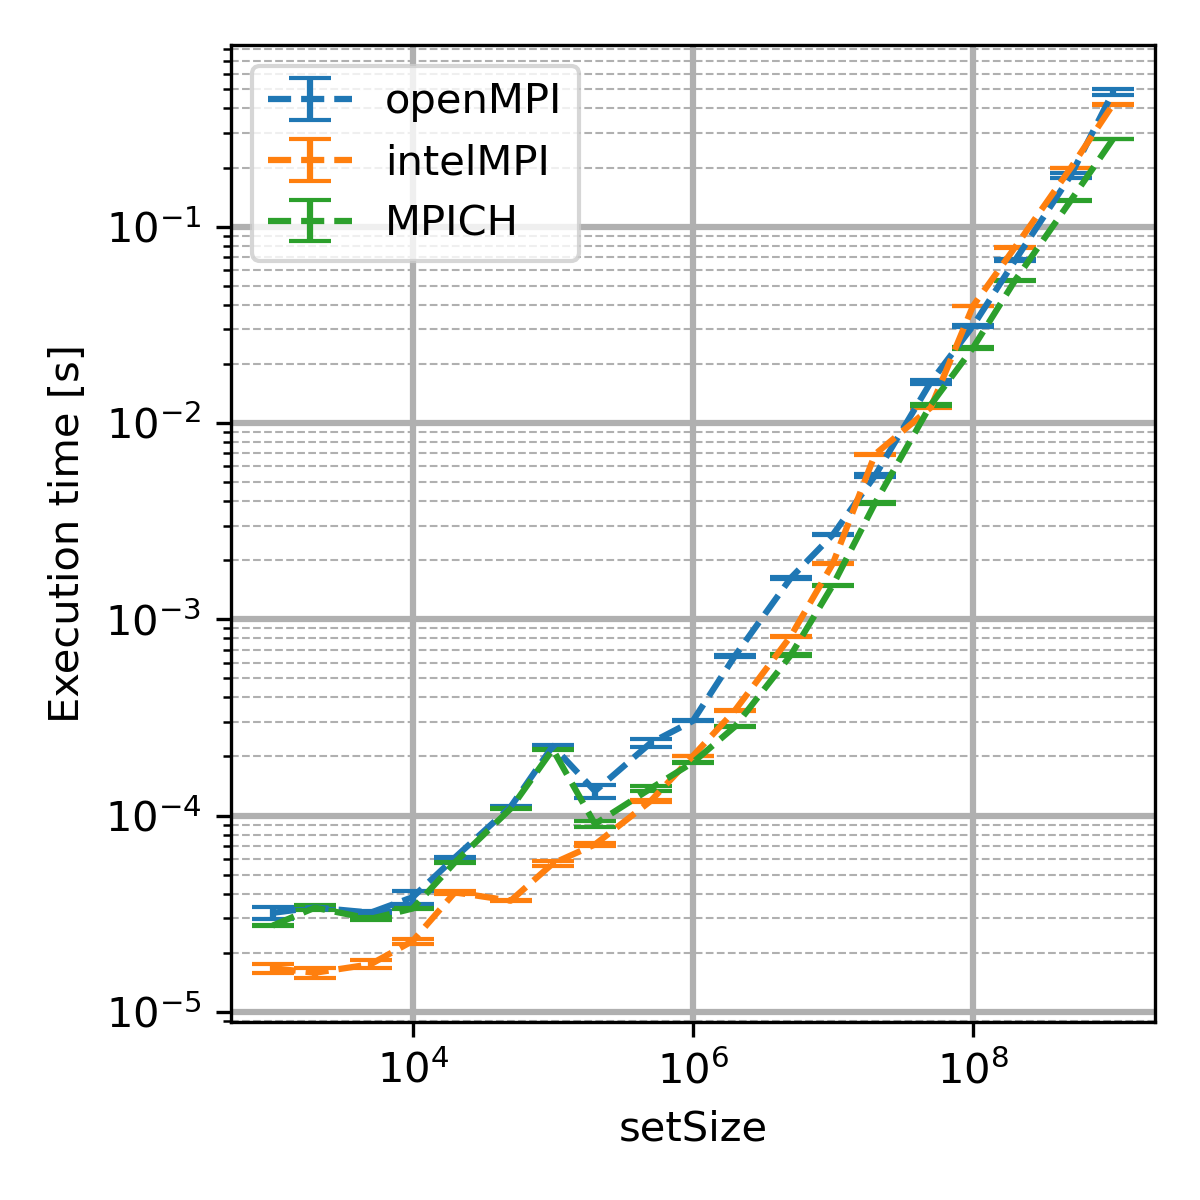
\includegraphics[width=\textwidth]{../plots/AllreduceLibs/32x32AllreduceLibs.png}
		\caption{$p=(32\times32)$}
		\label{fig:32x32}
	\end{subfigure}
	\hfill
	\begin{subfigure}[b]{0.45\textwidth}
		\centering
		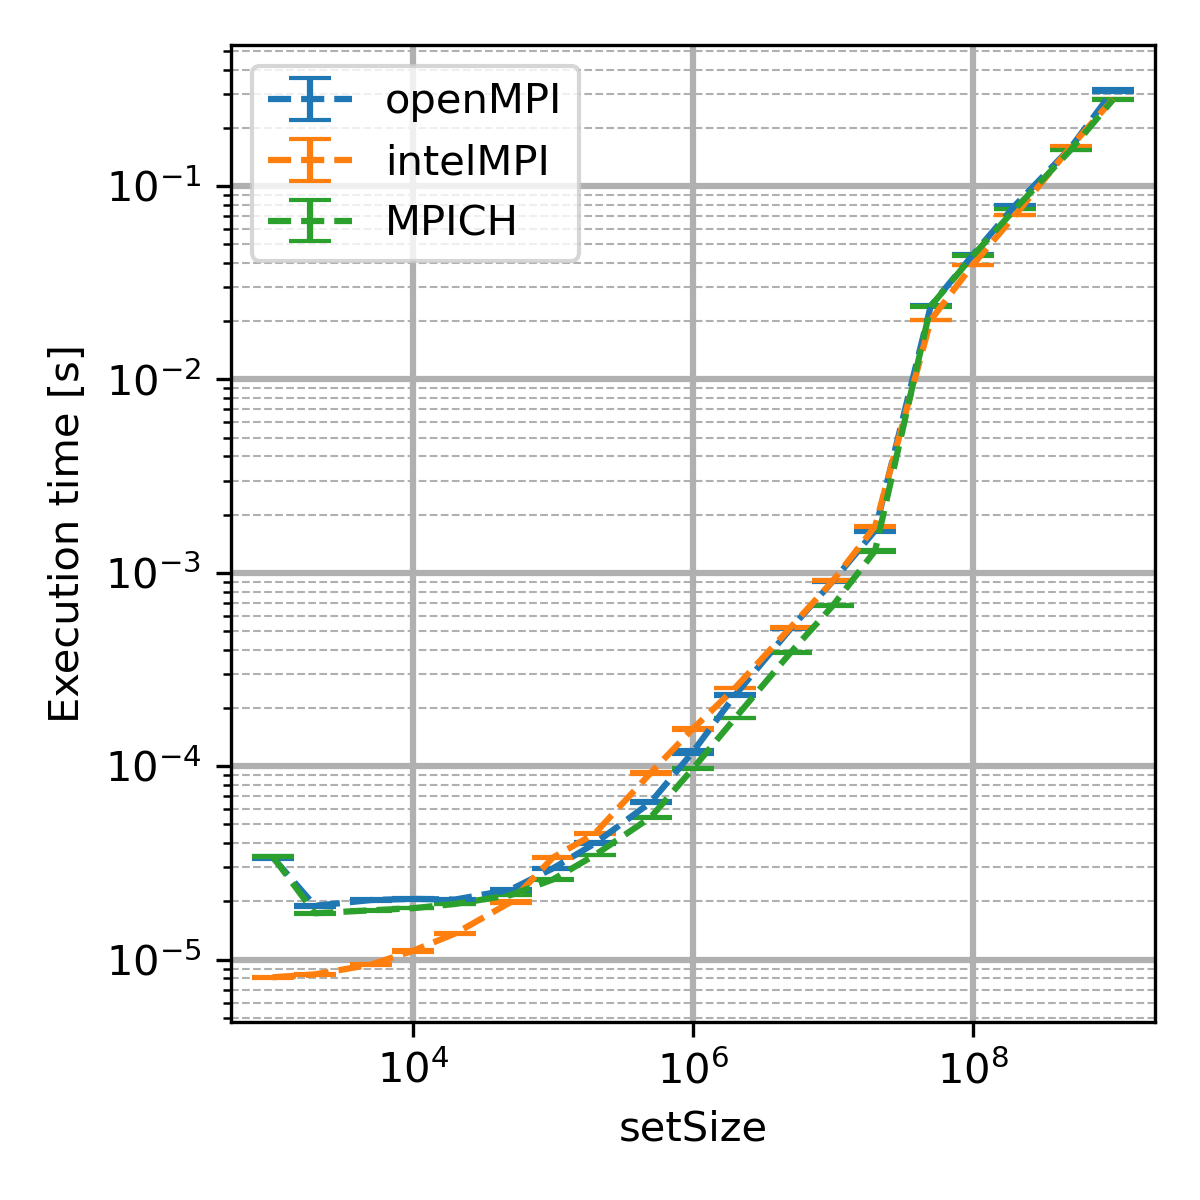
\includegraphics[width=\textwidth]{../plots/AllreduceLibs/32x1AllreduceLibs.png}
		\caption{$p=(32\times1)$}
		\label{fig:32x1}
	\end{subfigure}
	\begin{subfigure}[b]{0.45\textwidth}
		\centering
		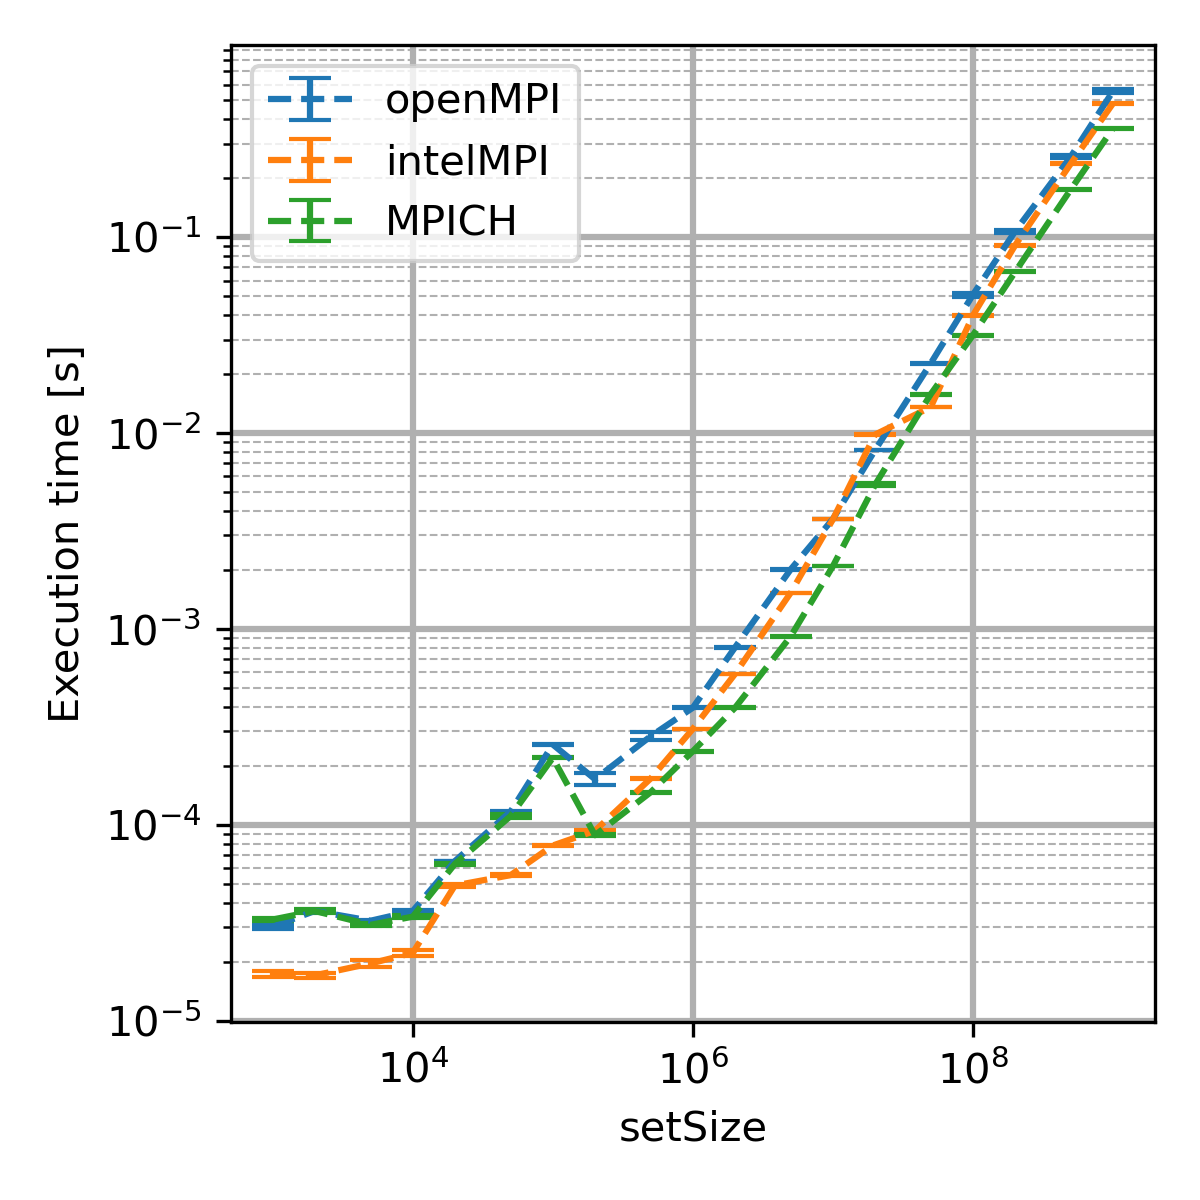
\includegraphics[width=\textwidth]{../plots/AllreduceLibs/36x32AllreduceLibs.png}
		\caption{$p=(36\times32)$}
		\label{fig:36x32}
	\end{subfigure}
	\hfill
	\begin{subfigure}[b]{0.45\textwidth}
		\centering
		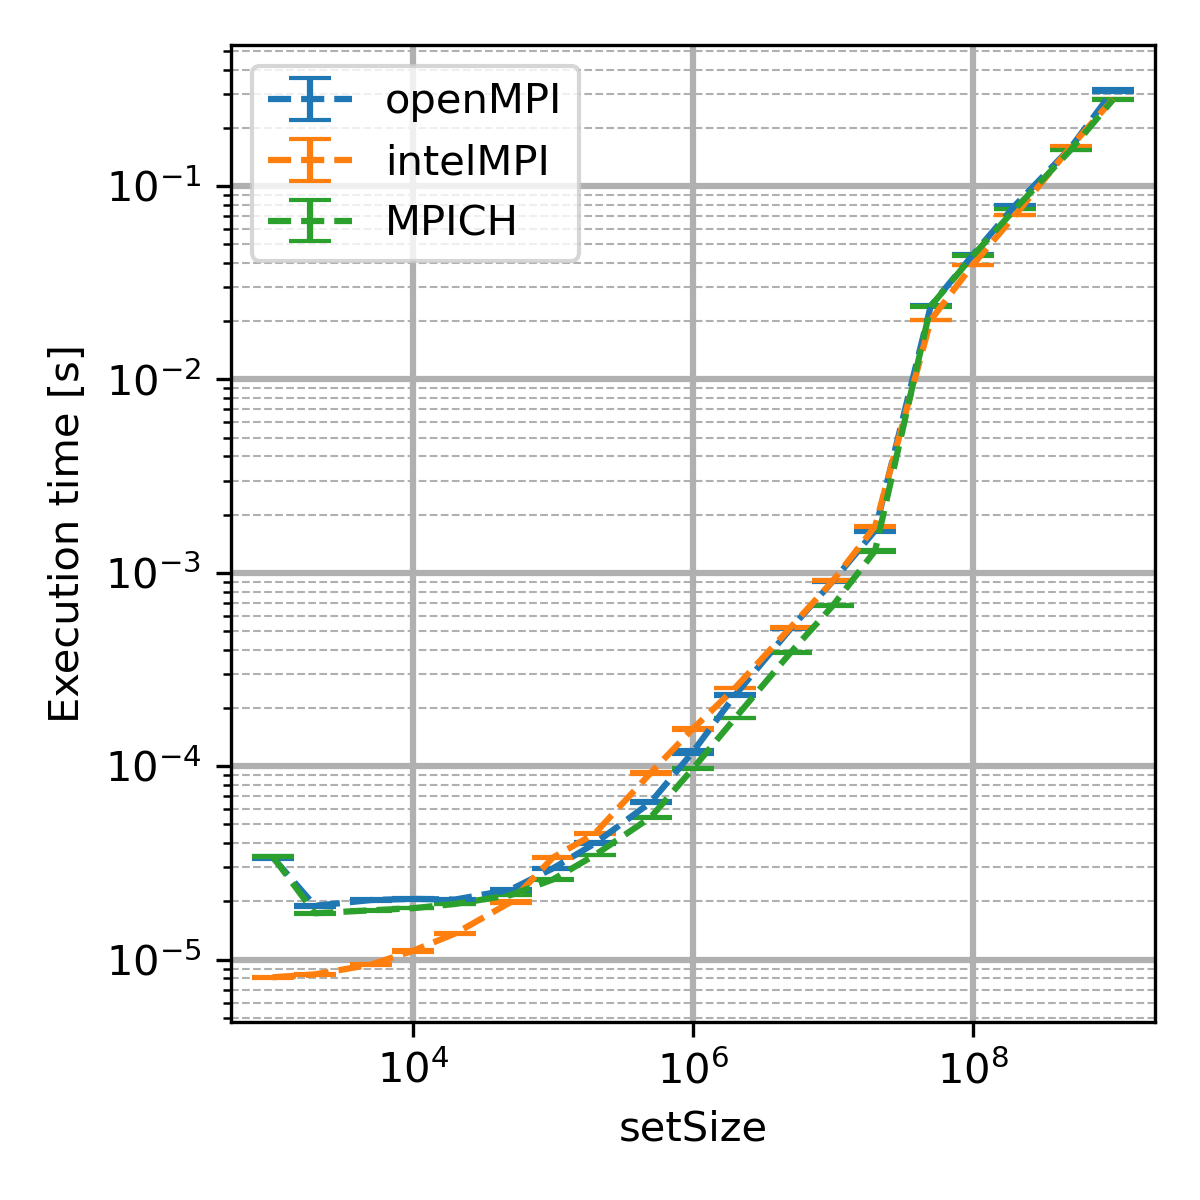
\includegraphics[width=\textwidth]{../plots/AllreduceLibs/32x1AllreduceLibs.png}
		\caption{$p=(36\times1)$}
		\label{fig:36x1}
	\end{subfigure}
	\caption{Benchmark of the Allreduce implementations provided by the different MPI libraries. Execution time $t$ is plotted against set size $|S|$. Four different processor layouts are shown (indicated by $p$).}
	\label{fig:AllreduceMPIlibs}
\end{figure}

\subsection{Foundation Allreduce algorithms}
Here the foundation algorithms are tested. There are three different implementations to test. The first two are based on the butterfly communication scheme and can therefore only work a number of processors that is a power of 2. These two implementations only differ in the rank ID mapping. The first one implements Algorithm \ref{algo:redScatterAndAllreduce} and is from now on referred as \texttt{Allreduce\_Butterfly}. The second one is the same algorithm but with a rank ID mapping where the ID is mapped to its bit reversal. This algorithm is from now on referred as \texttt{Allreduce\_Butterfly\_Reversed}. The third algorithm uses a shift based communication pattern, is the implementation of Algorithm \ref{algo:redScatterAndAllgatherShift} and is from now on called \texttt{Allreduce\_Shift}. This algorithm works correctly for an arbitrary number of processors. 


\section{Testing foundation Allgather against MPI-libraries} \label{sec:baseAllgather}

\section{Comparison of Proposed Algorithms Against Their Base Variant}
\subsection{$2^k$ Variant}
\subsection{Arbitrary Number of Processes Variant}
\subsection{Naive Variant}
\section{Performance Testing Using \gls{bfs} as Benchmark}
